% !TEX TS-program = LuaLaTeX+shellescape
% !TEX encoding = UTF-8 Unicode
\RequirePackage{luatex85}
\documentclass[crop=true]{standalone}
\usepackage{pgfplots}
\usepgfplotslibrary{fillbetween}
%\usetikzlibrary{angles}
\pgfplotsset{compat=1.15}
%\pdfminorversion=5 % to allow compression
%\pdfobjcompresslevel=5
%\pdfcompresslevel=14
%\pgfplotsset{
%	layers/my layer set/.define layer set={background,main,foreground}{},set layers=my layer set,}

\begin{document}
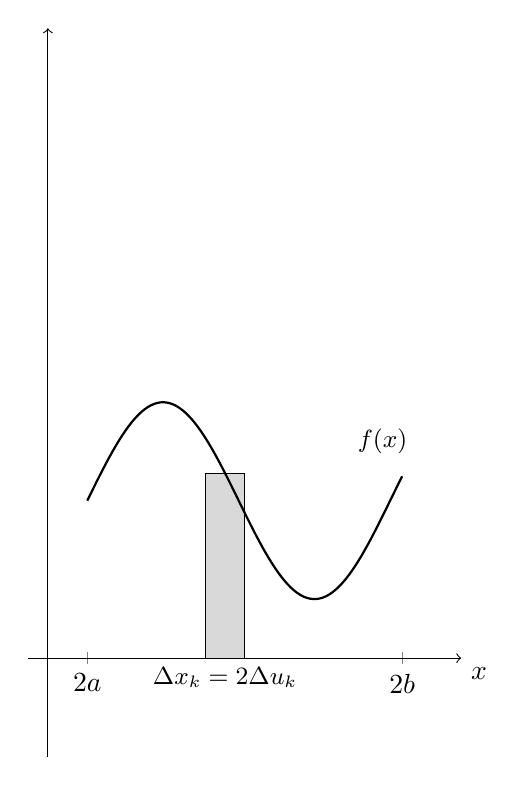
\begin{tikzpicture}
\begin{axis}[
axis lines = middle,
% unit vector ratio=1 1, 
% axis equal=false,
% scale=1.0, 
x = 2.5cm, 
y = 2.5cm, 
xmin=-0.1, xmax=2.1, ymin=-0.5, ymax=3.20, 
% grid = major,
xtick={0.2,1.8},
ytick={0},
xticklabels = {$2a$, $2b$},
yticklabels = {},
xlabel=$x$,
ylabel={}, 
xlabel style={below right},
ylabel style={above left},
axis line style = {->},
]

\pgfmathsetmacro{\a}{0.2} 
\pgfmathsetmacro{\b}{1.8}
\pgfmathtruncatemacro{\Nsub}{8} 
\pgfmathsetmacro{\h}{(\b-\a)/\Nsub}
\pgfmathtruncatemacro{\i}{3} 
\pgfmathsetmacro{\xleft}{\a+\i*\h}
\pgfmathsetmacro{\xright}{\a+(\i+1)*\h} 
\pgfmathsetmacro{\xmid}{\a+(\i+0.5)*\h}
\pgfmathsetmacro{\height}{(sin(deg(1.3*pi*(\xmid-0.2)))+1.6)/2} 
\fill[gray!30] (axis cs:{\xleft},{0}) rectangle (axis cs:{\xright},{\height}); 
\draw (axis cs:{\xleft},{0}) rectangle (axis cs:{\xright},{\height});

\addplot [style=thick, domain=0.2:1.8, samples=100] {(sin(deg(1.3*pi*(x-0.2)))+1.6)/2};

\node at (0.9, -0.1) {\small $\Delta x_k = 2\Delta u_k$};
\node at (1.7, 1.1) {\small $f(x)$};
\end{axis}
\end{tikzpicture}

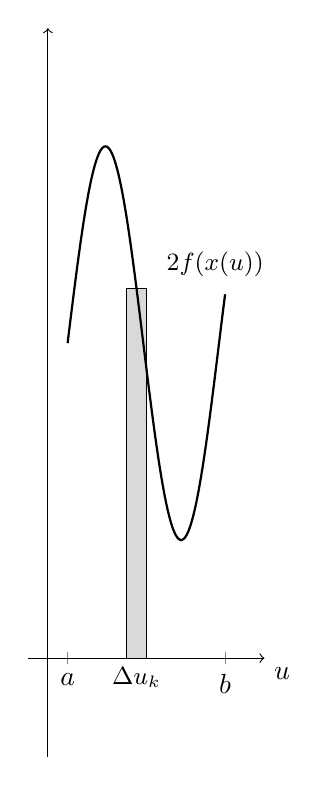
\begin{tikzpicture}
\begin{axis}[
axis lines = middle,
% unit vector ratio=1 1, 
% axis equal=false,
% scale=1.0, 
x = 2.5cm,
y = 2.5cm, 
xmin=-0.1, xmax=1.1, ymin=-0.5, ymax=3.20, 
% grid = major,
xtick={0.1,0.9},
ytick={0},
xticklabels = {$a$, $b$},
yticklabels = {},
xlabel=$u$,
ylabel={},
xlabel style={below right},
ylabel style={above left},
axis line style = {->},
]

\pgfmathsetmacro{\a}{0.1} 
\pgfmathsetmacro{\b}{0.9}
\pgfmathtruncatemacro{\Nsub}{8} 
\pgfmathsetmacro{\h}{(\b-\a)/\Nsub}
\pgfmathtruncatemacro{\i}{3} 
\pgfmathsetmacro{\xleft}{\a+\i*\h}
\pgfmathsetmacro{\xright}{\a+(\i+1)*\h} 
\pgfmathsetmacro{\xmid}{\a+(\i+0.5)*\h}
\pgfmathsetmacro{\height}{(sin(deg(1.3*pi*(2*\xmid-0.2)))+1.6)} 
\fill[gray!30] (axis cs:{\xleft},{0}) rectangle (axis cs:{\xright},{\height}); 
\draw (axis cs:{\xleft},{0}) rectangle (axis cs:{\xright},{\height});

\addplot [style=thick, domain=0.1:0.9, samples=100] {(sin(deg(1.3*pi*(2*x-0.2)))+1.6)};
\node at (0.45, -0.1) {\small $\Delta u_k$};
\node at (0.85, 2.0) {\small $2f(x(u))$};
\end{axis}
\end{tikzpicture}



\end{document}